\section{2. Дерева та ансамблі}

\markright{Частина 2}

На наступному кроці ми моделюємо SalePrice за допомогою дерев регресії,
використовуючи DecisionTreeRegressor з бібліотеки sklearn.tree.


\Needspace{167pt}

\subsection{2.а Критерій поділу}

\begin{taskstatement}Нехай GrLivArea буде першою змінною, яка використовується для
розщеплення (splitting). Запишіть відповідну задачу оптимізації
(мінімізацію суми квадратів залишків RSS для двох дочірніх вузлів) та
поясніть, як працює алгоритм жадібного пошуку точки розщеплення.
\end{taskstatement}

\par\medskip
Для першого розщеплення фіксуємо \(x_i=GrLivArea_i\) і розв'язуємо
\[\min_s\left[\sum_{i:x_i\le s}(y_i-\bar y_L(s))^2+\sum_{i:x_i>s}(y_i-\bar y_R(s))^2\right].\]
Тут \(x_i\) є житловою площею будинку \(i\), \(y_i\) його ціною, \(s\)
порогом, а \(\bar y_L(s)\) та \(\bar y_R(s)\) середніми цінами лівої та
правої груп. Обидві групи мають бути непорожніми. Для фіксованого порогу
саме середні мінімізують суму квадратів у групах.

Алгоритм сортує різні значення площі та перевіряє пороги посередині між
сусідніми різними значеннями. Розщеплення між однаковими значеннями не
допускається. Обираємо поріг із найменшим сумарним RSS дочірніх вузлів.
Пошук жадібний: він оптимізує лише поточний поділ, не перебираючи всі
можливі майбутні дерева.

У цьому пункті ознаку задано умовою. У повній моделі нижче CART сам
вибирає і ознаку, і поріг; її кореневий поділ не зобов'язаний
використовувати \texttt{GrLivArea}.


\Needspace{277pt}

\subsection{2.в Порядкові та категоріальні ознаки}

\begin{taskstatement}Тепер розгляньте змінну OverallQual. Вона приймає 10 різних
упорядкованих значень (від 1 до 10). Як алгоритм дерева на Python
визначає оптимальне розщеплення для такого типу дискретних або рангових
змінних? Опишіть логіку обробки категоріальних та порядкових ознак у
деревах.
\end{taskstatement}

\pythoncode{p2-c12}

\Needspace{46.8pt}

\resulttext{p2-c12-out0.txt}

\answerheading
Для \texttt{OverallQual} можливі поділи виду «оцінка не більша за поріг»
та «оцінка більша за поріг». Якщо присутні всі рівні від 1 до 10,
достатньо перевірити дев'ять меж: 1.5, 2.5, \ldots, 9.5. Вивід показує
фактичні рівні, кандидатів і обраний поділ. Обидві дочірні групи
складаються із суміжних рівнів порядкової шкали.

\texttt{DecisionTreeRegressor} обробляє числову порядкову ознаку через
порогові порівняння. Це використовує її порядок і не вимагає лінійного
зв'язку оцінки з ціною. Для номінальних категорій довільні числові коди
нав'язали б штучний порядок. Тому тут використовуємо
\texttt{OneHotEncoder}: поділ даммі за 0.5 відокремлює один рівень від
решти. Клас scikit-learn не перебирає довільні підмножини текстових
категорій автоматично.

Окреме дерево обрало поріг 7.5: оцінки до 7 включно потрапляють ліворуч,
від 8 праворуч. Середні ціни цих груп становлять приблизно 155840 та
299913 доларів.


\Needspace{332pt}

\subsection{2.г Обмеження розміру CART}

\begin{taskstatement}Очевидно, що без обмежень можна отримати дуже великі перенавчені дерева.
Стрижка дерев (tree pruning) допомагає досягти розумного розміру.
Підгоніть модель CART за допомогою DecisionTreeRegressor і обмежте її
так, щоб вона мала не більше 10 розщеплень (параметр
max\_leaf\_nodes=11).
\end{taskstatement}

\pythoncode{p2-c15}

\Needspace{95pt}
\begingroup\fontsize{7.5}{9.5}\selectfont\setlength{\tabcolsep}{2.5mm}\renewcommand{\arraystretch}{1.12}\par\noindent\begin{tabular}{|ll|}
\hline
 & Значення \\
\hline
Листків & 11 \\
Поділів & 10 \\
Глибина & 4 \\
Навчальна MSE, дол.\textasciicircum{}2 & 1.36773e+09 \\
Валідаційна MSE, дол.\textasciicircum{}2 & 1.58884e+09 \\
\hline
\end{tabular}
\par\endgroup


\begin{figure}[H]\centering
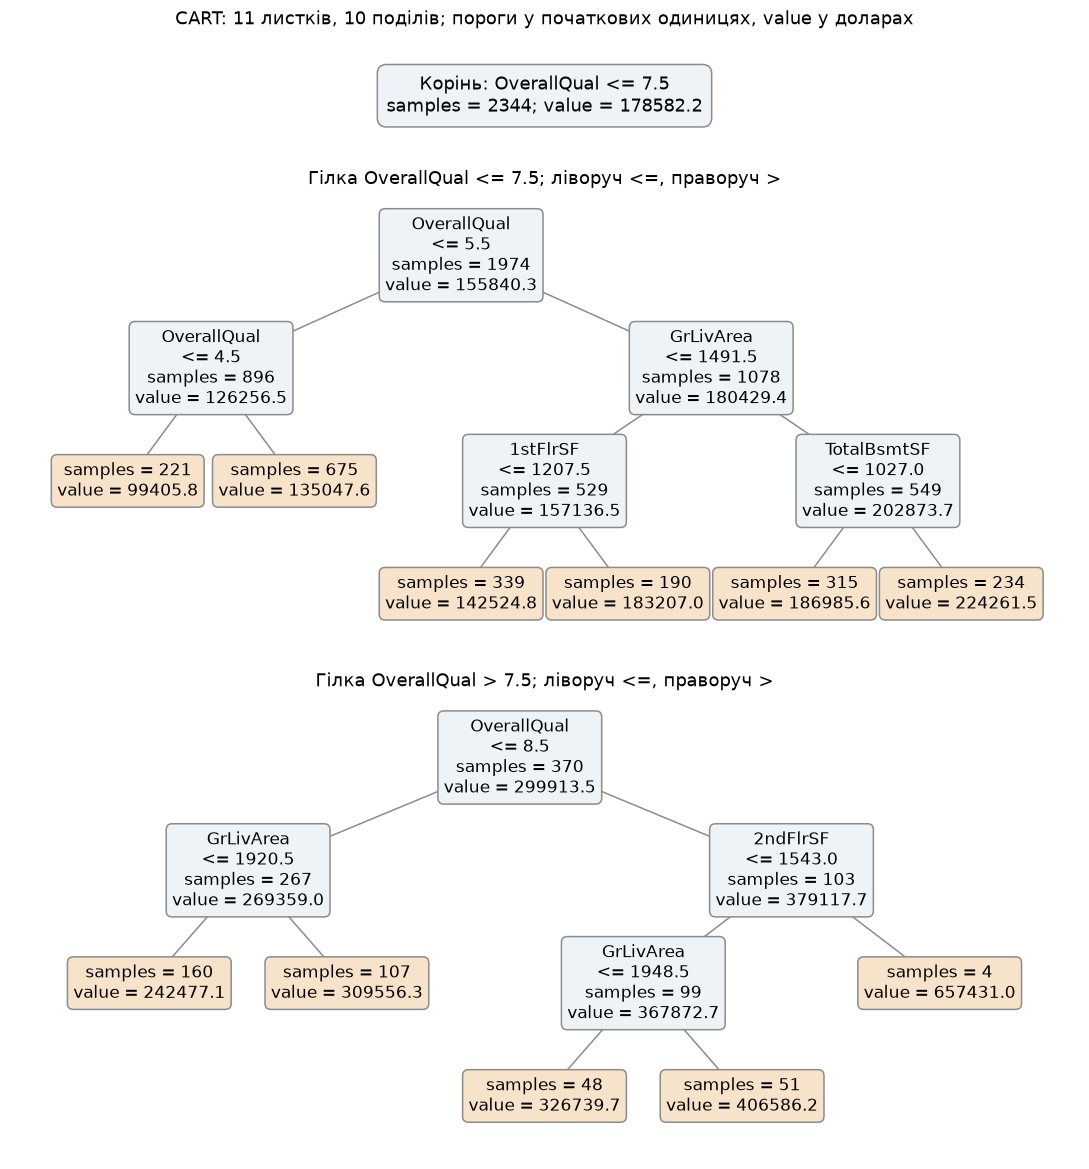
\includegraphics[width=1\linewidth,height=0.85\textheight,keepaspectratio]{../../figures/part2_cart.png}
\caption{Дерево CART із десятьма поділами. Пороги у початкових одиницях.}
\end{figure}

\answerheading
\texttt{max\_leaf\_nodes=11} обмежує дерево одинадцятьма листками. Кожен
бінарний поділ замінює один листок двома, тому кількість поділів
дорівнює кількості листків мінус один. Числовий вивід і схема показують
фактичний розмір дерева та його помилки.

Це обмеження росту під час навчання. На кожному кроці розщеплюється
доступний листок із найбільшим покращенням критерію. Подальше обрізання
через \texttt{ccp\_alpha} розглядаємо в наступному пункті. На рисунку
\texttt{samples} означає кількість навчальних будинків, а \texttt{value}
середню ціну у вузлі.

Отримано 11 листків, 10 поділів і глибину 4. Навчальна MSE становить
приблизно \(1.368\cdot10^9\), валідаційна \(1.589\cdot10^9\) дол.².
Обмеження листків виконано; воно не гарантує, що саме цей розмір є
найкращим.


\Needspace{323pt}

\subsection{2.д Обрізання дерева}

\begin{taskstatement}Знайдіть значення параметра складності (Cost-Complexity Pruning alpha,
ccp\_alpha) за допомогою методу cost\_complexity\_pruning\_path() для
дерева, навченого в попередньому пункті. Що це за параметр і що він
регулює? Що станеться з архітектурою дерева, якщо ми суттєво збільшимо
або зменшимо ccp\_alpha? Перевірте це експериментально на ваших даних.
\end{taskstatement}

\pythoncode{p2-c18}

\Needspace{19.2pt}

\resulttext{p2-c18-out0.txt}

\Needspace{173pt}
\begingroup\fontsize{7.5}{9.5}\selectfont\setlength{\tabcolsep}{1.5mm}\renewcommand{\arraystretch}{1.12}\par\noindent\begin{tabular}{|>{\raggedright\arraybackslash}p{20.53mm}>{\raggedright\arraybackslash}p{16.01mm}>{\raggedright\arraybackslash}p{16.01mm}>{\raggedright\arraybackslash}p{29.30mm}>{\raggedright\arraybackslash}p{30.81mm}>{\raggedright\arraybackslash}p{34.33mm}|}
\hline
ccp\_alpha & Листків & Глибина & Навчальна MSE, дол.\textasciicircum{}2 & Валідаційна MSE, дол.\textasciicircum{}2 & Зважена неоднорідність шляху \\
\hline
0 & 11 & 4 & 1.36773e+09 & 1.58884e+09 & 1.36773e+09 \\
6.7256e+07 & 10 & 4 & 1.43499e+09 & 1.73846e+09 & 1.43499e+09 \\
7.9589e+07 & 9 & 4 & 1.51458e+09 & 1.83625e+09 & 1.51458e+09 \\
8.59704e+07 & 8 & 3 & 1.60055e+09 & 1.93902e+09 & 1.60055e+09 \\
9.023e+07 & 7 & 3 & 1.69078e+09 & 2.01528e+09 & 1.69078e+09 \\
1.23087e+08 & 6 & 3 & 1.81386e+09 & 2.21125e+09 & 1.81386e+09 \\
1.37522e+08 & 5 & 3 & 1.95139e+09 & 2.27441e+09 & 1.95139e+09 \\
2.40431e+08 & 4 & 2 & 2.19182e+09 & 2.60159e+09 & 2.19182e+09 \\
3.82003e+08 & 3 & 2 & 2.57382e+09 & 3.33575e+09 & 2.57382e+09 \\
6.12612e+08 & 2 & 1 & 3.18643e+09 & 4.08078e+09 & 3.18643e+09 \\
2.75931e+09 & 1 & 0 & 5.94574e+09 & 8.14008e+09 & 5.94574e+09 \\
\hline
\end{tabular}
\par\endgroup


\begin{figure}[H]\centering
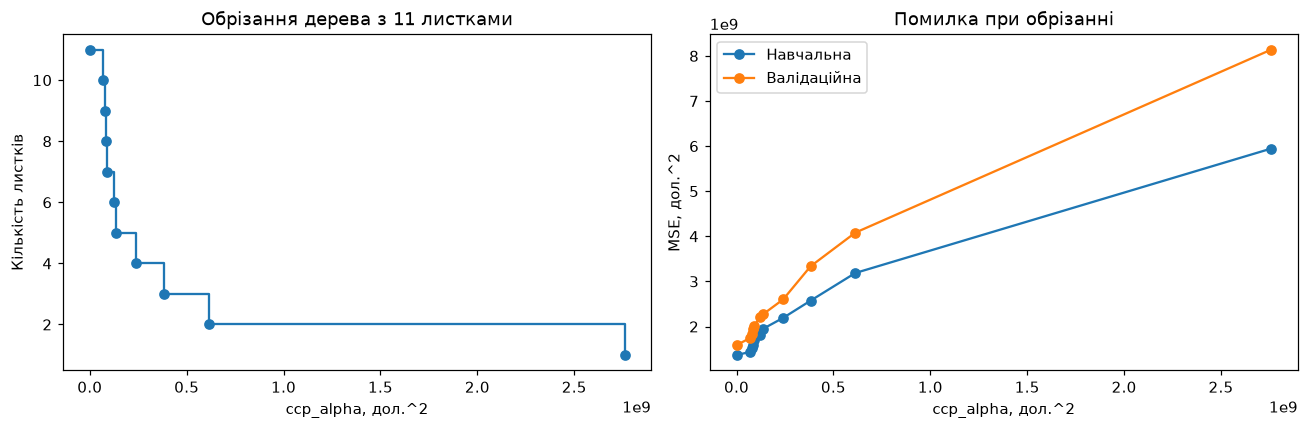
\includegraphics[width=1\linewidth,height=0.85\textheight,keepaspectratio]{../../figures/part2_pruning.png}
\caption{Розмір дерева та помилка при обрізанні.}
\end{figure}

\answerheading
Метод \texttt{cost\_complexity\_pruning\_path()} дає послідовність
критичних штрафів, за яких видаляються гілки. Це набір кандидатів, а не
автоматичний вибір оптимального штрафу.

У scikit-learn мінімізується \(R_\alpha(T)=R(T)+\alpha|T|\), де \(T\) є
деревом, \(|T|\) кількістю листків, \(\alpha\) параметром
\texttt{ccp\_alpha}, а \(R(T)\) сумою зважених неоднорідностей листків.
Для критерію \texttt{squared\_error} без ваг \(R(T)=RSS(T)/n\), де
\(RSS(T)\) сума квадратів навчальних залишків, \(n\) кількість
навчальних будинків. Тому \texttt{ccp\_alpha} має шкалу дол.²; у формулі
зі звичайною сумою RSS штраф потрібно помножити на \(n\).

За нульового штрафу залишається початкове дерево, обмежене одинадцятьма
листками. Збільшення штрафу послідовно прибирає гілки; останній кандидат
залишає лише корінь, що прогнозує навчальне середнє ціни. Зменшення
штрафу повертає більш детальне дерево, але не скасовує обмеження
\texttt{max\_leaf\_nodes=11}. Навчальна помилка при обрізанні не
зменшується; поведінку валідаційної перевіряємо за таблицею.

Результати після обчислень

За нульового штрафу дерево мало 11 листків і глибину 4. Перший додатний
поріг, приблизно \(6.726\cdot10^7\), зменшив кількість листків до 10. За
штрафу близько \(2.759\cdot10^9\) залишився один листок, а глибина стала
0. На перевірених значеннях валідаційна MSE зростала, тому додаткове
обрізання не покращило прогноз на цій валідаційній вибірці.


\Needspace{310pt}

\subsection{2.е Покращення в корені}

\begin{taskstatement}Перевірте значення покращення (improvement / зменшення критерію
неоднорідності) у першому розщепленні дерева. Поясніть концепцію
інформаційного прибутку (impurity reduction) та наведіть числовий вираз,
за яким воно обчислюється в scikit-learn для першого вузла.
\end{taskstatement}

\pythoncode{p2-c21}

\Needspace{19.2pt}

\resulttext{p2-c21-out0.txt}

\Needspace{69pt}
\begingroup\fontsize{7.5}{9.5}\selectfont\setlength{\tabcolsep}{2.5mm}\renewcommand{\arraystretch}{1.12}\par\noindent\begin{tabular}{|lll|}
\hline
Вузол & Кількість & MSE, дол.\textasciicircum{}2 \\
\hline
Корінь & 2344 & 5.94574e+09 \\
Лівий & 1974 & 2.29321e+09 \\
Правий & 370 & 7.95189e+09 \\
\hline
\end{tabular}
\par\endgroup


\Needspace{37.599999999999994pt}

\resulttext{p2-c21-out2.txt}

\answerheading
Інформаційний прибуток у корені показує, наскільки після поділу
зменшується середній квадрат відхилень цін від середнього свого вузла.
Від MSE кореня віднімаємо зважену MSE дочірніх вузлів.
\[\Delta=I-\frac{N_L}{N}I_L-\frac{N_R}{N}I_R.\] Тут \(\Delta\) є
покращенням, \(I\), \(I_L\) та \(I_R\) є MSE кореня, лівого й правого
вузлів, а \(N\), \(N_L\) та \(N_R\) позначають кількість навчальних
будинків у цих вузлах.

У корені обрано поділ \texttt{OverallQual\ ≤\ 7.5} у початковій шкалі.
Підставляємо значення зі збереженого виводу.
\[\Delta\approx\left(5.94574-\frac{1974}{2344}\cdot2.29321-\frac{370}{2344}\cdot7.95189\right)\cdot10^9\approx2.7593\cdot10^9\ \text{дол.}^2.\]
MSE правого вузла вища за MSE кореня. Проте в ньому лише 370 із 2344
будинків, і зважена MSE двох дочірніх вузлів після поділу зменшилася.


\Needspace{418pt}

\subsection{2.ж Важливості дерева та коефіцієнти}

\begin{taskstatement}Обчисліть важливість ознак (feature\_importances\_) для дерева регресії
та порівняйте топ-10 результатів із коефіцієнтами, отриманими в регресії
ласо та класичній лінійній регресії.
\end{taskstatement}

\pythoncode{p2-c24}

\Needspace{37.599999999999994pt}

\resulttext{p2-c24-out0.txt}

\Needspace{160pt}
\begingroup\fontsize{7.5}{9.5}\selectfont\setlength{\tabcolsep}{2.5mm}\renewcommand{\arraystretch}{1.12}\par\noindent\begin{tabular}{|llll|}
\hline
Ознака & Lasso, коеф. & OLS, коеф. & CART MDI \\
\hline
Overall\allowbreak{}Qual & 14157.1 & 8711.49 & 0.8397 \\
Gr\allowbreak{}Liv\allowbreak{}Area & 23057.6 & 16429.2 & 0.0940963 \\
2nd\allowbreak{}Flr\allowbreak{}SF & 4383.1 & 13632.9 & 0.0300397 \\
1st\allowbreak{}Flr\allowbreak{}SF & 0 & 6470.09 & 0.018779 \\
Total\allowbreak{}Bsmt\allowbreak{}SF & 4197.38 & 9661.19 & 0.0173851 \\
Lot\allowbreak{}Frontage & -1624.16 & 1350.95 & 0 \\
Lot\allowbreak{}Area & 3303.43 & 5462.63 & 0 \\
Overall\allowbreak{}Cond & 6306.27 & 6698.35 & 0 \\
Year\allowbreak{}Built & 9510.14 & 12549.5 & 0 \\
Year\allowbreak{}Remod\allowbreak{}Add & 2077.11 & 1021.81 & 0 \\
\hline
\end{tabular}
\par\endgroup


\Needspace{19.2pt}

\resulttext{p2-c24-out2.txt}

\Needspace{160pt}
\begingroup\fontsize{7.5}{9.5}\selectfont\setlength{\tabcolsep}{2.5mm}\renewcommand{\arraystretch}{1.12}\par\noindent\begin{tabular}{|lll|}
\hline
CART MDI & Lasso за модулем & OLS за модулем \\
\hline
Overall\allowbreak{}Qual & Pool\allowbreak{}QC\_Gd & Roof\allowbreak{}Matl\_Membran \\
Gr\allowbreak{}Liv\allowbreak{}Area & Misc\allowbreak{}Feature\_Gar2 & Roof\allowbreak{}Matl\_Wd\allowbreak{}Shngl \\
2nd\allowbreak{}Flr\allowbreak{}SF & Roof\allowbreak{}Matl\_Wd\allowbreak{}Shngl & Roof\allowbreak{}Matl\_Metal \\
1st\allowbreak{}Flr\allowbreak{}SF & Neighbor\-hood\_Stone\allowbreak{}Br & Roof\allowbreak{}Matl\_Roll \\
Total\allowbreak{}Bsmt\allowbreak{}SF & Neighbor\-hood\_No\allowbreak{}Ridge & Roof\allowbreak{}Matl\_Wd\allowbreak{}Shake \\
Lot\allowbreak{}Frontage & Neighbor\-hood\_Nridg\allowbreak{}Ht & Roof\allowbreak{}Matl\_Comp\allowbreak{}Shg \\
Lot\allowbreak{}Area & Kitchen\allowbreak{}Qual\_TA & Roof\allowbreak{}Matl\_Tar\&Grv \\
Overall\allowbreak{}Cond & Neighbor\-hood\_Grn\allowbreak{}Hill & Misc\allowbreak{}Feature\_Othr \\
Year\allowbreak{}Built & Kitchen\allowbreak{}Qual\_Gd & Misc\allowbreak{}Feature\_Gar2 \\
Year\allowbreak{}Remod\allowbreak{}Add & Gr\allowbreak{}Liv\allowbreak{}Area & Misc\allowbreak{}Feature\_Shed \\
\hline
\end{tabular}
\par\endgroup


\answerheading
MDI підсумовує зважене зменшення неоднорідності в усіх поділах за
ознакою та нормує внески так, щоб їхня сума дорівнювала одиниці. У
таблиці зіставляємо MDI десяти ознак дерева з коефіцієнтами тих самих
ознак у Lasso й МНК. MDI безрозмірна й показує внесок у поділи. Знак
коефіцієнта показує напрям зміни прогнозу лінійної моделі за незмінних
інших ознак.

Лише п'ять ознак мають додатну MDI. Решта рядків топ-10 мають нульову
MDI нарівні з іншими невикористаними ознаками. Найвищі MDI у
\texttt{OverallQual} (0.8397) та \texttt{GrLivArea} (0.09410), і для
обох коефіцієнти Lasso й МНК додатні. Дерево використало
\texttt{1stFlrSF}, а Lasso оцінило її коефіцієнт нулем.


\Needspace{497pt}

\subsection{2.і Помилка ансамблів}

\begin{taskstatement}Використовуйте беггінг (BaggingRegressor) та випадковий ліс
(RandomForestRegressor) для прогнозування SalePrice. Побудуйте графік
залежності середньоквадратичної помилки (MSE) на навчальній та
валідаційній вибірках від кількості базових дерев (n\_estimators).
Прокоментуйте поведінку обох кривих на графіку.
\end{taskstatement}

\pythoncode{p2-c33}

\Needspace{19.2pt}

\resulttext{p2-c33-out0.txt}

\Needspace{212pt}
\begingroup\fontsize{7.5}{9.5}\selectfont\setlength{\tabcolsep}{2.5mm}\renewcommand{\arraystretch}{1.12}\par\noindent\begin{tabular}{|llll|}
\hline
Модель & Дерев & Навчальна MSE, дол.\textasciicircum{}2 & Валідаційна MSE, дол.\textasciicircum{}2 \\
\hline
Bagging & 1 & 6.53192e+08 & 1.53168e+09 \\
Bagging & 5 & 2.05021e+08 & 8.4875e+08 \\
Bagging & 10 & 1.68949e+08 & 7.66191e+08 \\
Bagging & 25 & 1.22267e+08 & 7.41785e+08 \\
Bagging & 50 & 1.07443e+08 & 7.22265e+08 \\
Bagging & 100 & 1.00961e+08 & 7.05429e+08 \\
Bagging & 200 & 9.85243e+07 & 7.0914e+08 \\
Random Forest & 1 & 6.40523e+08 & 2.56631e+09 \\
Random Forest & 5 & 2.00007e+08 & 9.50028e+08 \\
Random Forest & 10 & 1.50852e+08 & 8.11277e+08 \\
Random Forest & 25 & 1.21991e+08 & 7.24634e+08 \\
Random Forest & 50 & 1.05962e+08 & 7.25563e+08 \\
Random Forest & 100 & 9.81004e+07 & 6.97905e+08 \\
Random Forest & 200 & 9.43458e+07 & 7.18452e+08 \\
\hline
\end{tabular}
\par\endgroup


\begin{figure}[H]\centering
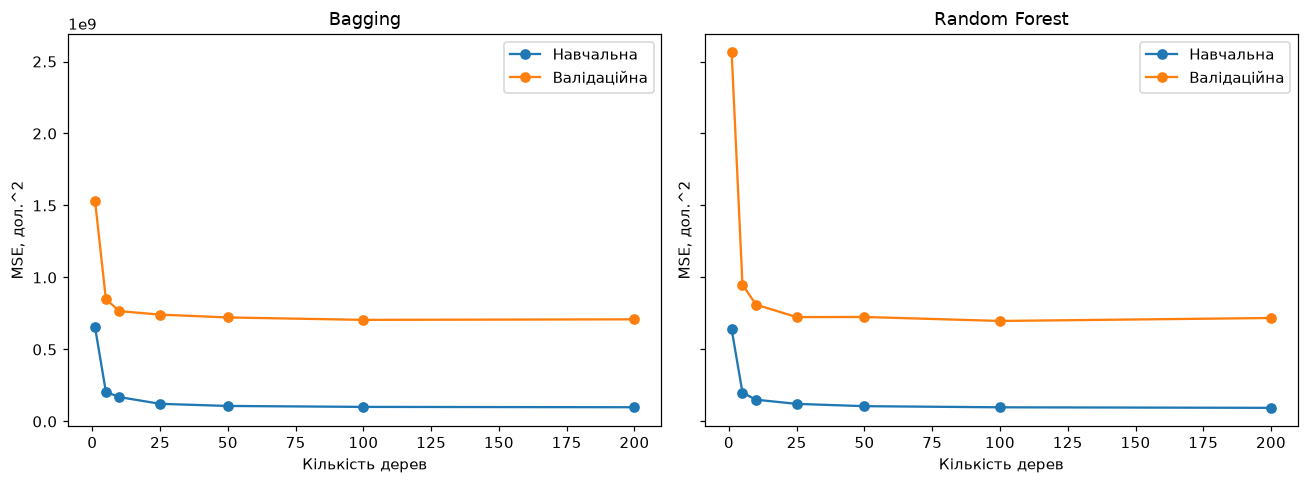
\includegraphics[width=1\linewidth,height=0.85\textheight,keepaspectratio]{../../figures/part2_ensemble_mse.png}
\caption{Навчальна й валідаційна MSE залежно від кількості дерев.}
\end{figure}

\Needspace{56pt}
\begingroup\fontsize{7.5}{9.5}\selectfont\setlength{\tabcolsep}{2.5mm}\renewcommand{\arraystretch}{1.12}\par\noindent\begin{tabular}{|lll|}
\hline
Модель & Початок плато на сітці & MSE при 200 деревах, дол.\textasciicircum{}2 \\
\hline
Bagging & 100 & 7.0914e+08 \\
Random Forest & 25 & 7.18452e+08 \\
\hline
\end{tabular}
\par\endgroup


\answerheading
Обидва ансамблі усереднюють прогнози дерев, навчених на вибірках із
поверненням. У випадковому лісі кожен вузол розглядає випадкову
підмножину ознак, тому дерева можуть давати менш схожі прогнози.

Початком плато називаємо найменшу перевірену кількість дерев, від якої
всі показані валідаційні MSE не більш ніж на 1\% перевищують MSE цієї
моделі при 200 деревах.

Навчальна MSE спадала на всій перевіреній сітці в обох моделей і
залишалася нижчою за валідаційну. Валідаційна MSE найбільше впала від 1
до 5 дерев. В обох моделей вона була найменшою при 100 деревах і трохи
зросла при 200. За критерієм 1\% плато починається зі 100 дерев для
беггінгу і з 25 для випадкового лісу. При 200 деревах валідаційна MSE
становить \(7.0914\cdot10^8\) дол.² для беггінгу та \(7.1845\cdot10^8\)
дол.² для лісу.


\Needspace{523pt}

\subsection{2.к Час та важливості моделей}

\begin{taskstatement}Порівняйте час виконання (time.time()) обох ансамблевих підходів. Чому
випадковий ліс зазвичай обчислювально швидший і потребує менше дерев
порівняно з чистим беггінгом над глибокими деревами? Перевірте
вбудований метод розрахунку важливості ознак для RandomForestRegressor
(MDI або permutation importance). Зробіть фінальну порівняльну таблицю
важливостей змінних для всіх моделей: Lasso, OLS, одиночне дерево та
Random Forest.
\end{taskstatement}

\pythoncode{p2-c36}

\Needspace{19.2pt}

\resulttext{p2-c36-out0.txt}

\Needspace{108pt}
\begingroup\fontsize{7.5}{9.5}\selectfont\setlength{\tabcolsep}{2.5mm}\renewcommand{\arraystretch}{1.12}\par\noindent\begin{tabular}{|lll|}
\hline
Повтор & Модель & Час навчання, с \\
\hline
1 & Bagging & 5.72391 \\
1 & Random Forest & 2.11956 \\
2 & Random Forest & 2.10959 \\
2 & Bagging & 5.63344 \\
3 & Bagging & 5.63201 \\
3 & Random Forest & 2.12593 \\
\hline
\end{tabular}
\par\endgroup


\Needspace{56pt}
\begingroup\fontsize{7.5}{9.5}\selectfont\setlength{\tabcolsep}{2.5mm}\renewcommand{\arraystretch}{1.12}\par\noindent\begin{tabular}{|llll|}
\hline
Модель & median & min & max \\
\hline
Bagging & 5.63344 & 5.63201 & 5.72391 \\
Random Forest & 2.11956 & 2.10959 & 2.12593 \\
\hline
\end{tabular}
\par\endgroup


\Needspace{28.4pt}

\resulttext{p2-c36-out3.txt}

\Needspace{290pt}
\begingroup\fontsize{7.5}{9.5}\selectfont\setlength{\tabcolsep}{2.5mm}\renewcommand{\arraystretch}{1.12}\par\noindent\begin{tabular}{|lllll|}
\hline
Ознака & Lasso, коеф. & OLS, коеф. & CART MDI & Random Forest MDI \\
\hline
Overall\allowbreak{}Qual & 14157.1 & 8711.49 & 0.8397 & 0.286514 \\
Gr\allowbreak{}Liv\allowbreak{}Area & 23057.6 & 16429.2 & 0.0940963 & 0.104882 \\
Garage\allowbreak{}Cars & 6388.78 & 3417.26 & 0 & 0.101298 \\
Year\allowbreak{}Built & 9510.14 & 12549.5 & 0 & 0.0718618 \\
Total\allowbreak{}Bsmt\allowbreak{}SF & 4197.38 & 9661.19 & 0.0173851 & 0.0483594 \\
Exter\allowbreak{}Qual\_TA & -10256 & -18206.5 & 0 & 0.0451815 \\
Garage\allowbreak{}Area & 589.571 & 2437.46 & 0 & 0.04317 \\
1st\allowbreak{}Flr\allowbreak{}SF & 0 & 6470.09 & 0.018779 & 0.0391335 \\
2nd\allowbreak{}Flr\allowbreak{}SF & 4383.1 & 13632.9 & 0.0300397 & 0.0225395 \\
Full\allowbreak{}Bath & 2620.66 & 1406.64 & 0 & 0.020463 \\
Bsmt\allowbreak{}Fin\allowbreak{}SF1 & 4262.43 & 9812.54 & 0 & 0.0197775 \\
Lot\allowbreak{}Area & 3303.43 & 5462.63 & 0 & 0.0188103 \\
Year\allowbreak{}Remod\allowbreak{}Add & 2077.11 & 1021.81 & 0 & 0.0122537 \\
Fireplaces & 3818.73 & 3757.38 & 0 & 0.0113411 \\
Kitchen\allowbreak{}Qual\_TA & -24421.7 & -24433.6 & 0 & 0.0099555 \\
Fireplace\allowbreak{}Qu\_NA & -0 & -1791.63 & 0 & 0.00784692 \\
Mas\allowbreak{}Vnr\allowbreak{}Area & 2600.72 & 3286.45 & 0 & 0.00765501 \\
Foundation\_PConc & 2483.76 & 1431.63 & 0 & 0.00656926 \\
Lot\allowbreak{}Frontage & -1624.16 & 1350.95 & 0 & 0.00587695 \\
Bsmt\allowbreak{}Unf\allowbreak{}SF & -0 & 744.428 & 0 & 0.00550854 \\
\hline
\end{tabular}
\par\nopagebreak\vspace{1pt}{\itshape\color{black!60}Скорочено: із 294 ознак показано 20 з найбільшою MDI випадкового лісу; решта 274 мають меншу MDI.}
\par\endgroup


\Needspace{19.2pt}

\resulttext{p2-c36-out5.txt}

\begin{figure}[H]\centering
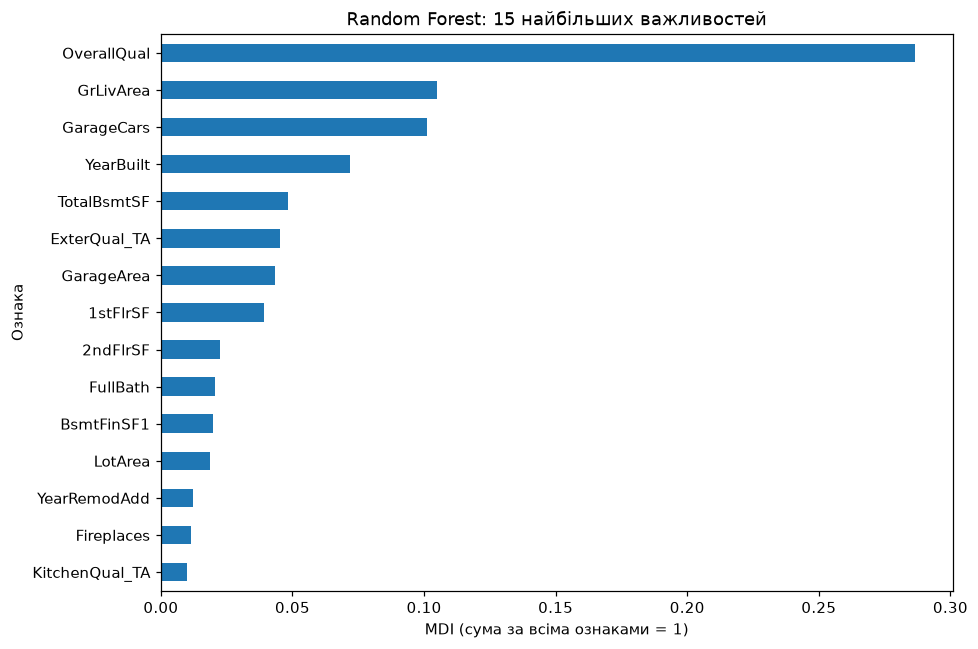
\includegraphics[width=1\linewidth,height=0.85\textheight,keepaspectratio]{../../figures/part2_forest_importance.png}
\caption{П’ятнадцять найбільших важливостей випадкового лісу.}
\end{figure}

У цьому запуску медіанний час навчання становить 5.633 с для беггінгу та
2.120 с для випадкового лісу. Ліс швидший приблизно у 2.66 раза. Це
підтверджує початкове очікування для заданих налаштувань.


\answerheading
Через \texttt{time.time()} вимірюємо час навчання з нуля. Для обох
методів використовуємо 200 глибоких дерев, ті самі дані й один потік.
Порівнюємо медіани трьох повторів із чергуванням порядку.

Беггінг розглядає всі ознаки у вузлі, а ліс із
\texttt{max\_features=1/3} зазвичай перевіряє менше кандидатів, тому
кожен поділ можна знайти швидше. Випадковий вибір ознак також зменшує
подібність дерев. Усереднення менш схожих прогнозів може стабілізувати
помилку за меншої кількості дерев.

Щоб перевірити MDI лісу, усереднюємо важливості дерев із поділами,
нормуємо їхню суму до одиниці й порівнюємо значення для кожної ознаки з
\texttt{feature\_importances\_}. Фінальна таблиця зіставляє коефіцієнти
Lasso й МНК із MDI одиночного дерева та лісу.

За критерієм 1\% із 2.і ліс досяг плато раніше за беггінг, хоча при 200
деревах його валідаційна MSE трохи вища. Найвищі MDI лісу мають
\texttt{OverallQual} (0.2865), \texttt{GrLivArea} (0.1049) і
\texttt{GarageCars} (0.1013). Частка \texttt{OverallQual} у лісі менша,
ніж в одиночному дереві, де її MDI становить 0.8397.

